\documentclass[10pt,a4paper]{article}
\usepackage[T1]{fontenc}
\usepackage[utf8]{inputenc}
\usepackage[spanish,es-tabla,es-nodecimaldot]{babel}
\usepackage{mathpazo}
\usepackage[scaled=0.9]{beramono}
\usepackage{microtype}
\usepackage[a4paper,margin=2.4cm]{geometry}
\usepackage{amsmath,amssymb}
\usepackage{booktabs}
\usepackage{graphicx}
\usepackage{tabularx}
\usepackage{caption}
\usepackage{fancyhdr}
\usepackage{titlesec}
\usepackage{tikz}
\usetikzlibrary{arrows.meta,positioning,babel}
\usepackage[hidelinks]{hyperref}

\captionsetup{font=small,labelfont=bf}
\titlespacing*{\section}{0pt}{2.2ex plus .5ex}{1.0ex}
\titlespacing*{\subsection}{0pt}{1.8ex plus .4ex}{0.8ex}
\setlength{\parskip}{0.25ex}
\pagestyle{fancy}
\fancyhf{}
\lhead{\small OII464: tercer informe}
\rhead{\small José Lara Arce}
\cfoot{\thepage}

\DeclareMathOperator*{\maxop}{m\acute{a}x}
\DeclareMathOperator*{\minop}{m\acute{\imath}n}
\newcommand{\Cmax}{C_{\text{máx}}}
\newcommand{\dc}{{,}}% coma decimal en modo matemático

\begin{document}

\begin{center}
{\LARGE\bfseries Planificación quirúrgica con dPSO\\[2pt]
y control aprendido de la perturbación en dos niveles\par}
\vspace{8pt}
{\large José Lara Arce}\\[2pt]
{\small Escuela de Ingeniería Informática, Pontificia Universidad Católica de Valparaíso\\
OII464: Desarrollo de Diseños Híbridos para Optimización\\
Profesor Emanuel Vega}
\end{center}

\begin{abstract}
\noindent
La planificación de cirugías electivas exige coordinar quirófanos y personal, respetando la
precedencia entre anestesia y cirugía. Las metaheurísticas aplicadas a este problema fijan sus
parámetros antes de ejecutar, y el control aprendido se ha estudiado sobre todo para elegir
operadores en algoritmos evolutivos. Proponemos añadir a la optimización discreta por enjambre
de partículas (dPSO) un control de la perturbación en dos niveles. Un bandido multibrazo elige
cada cinco iteraciones la probabilidad de mutar una partícula, y otro elige en cada mutación el
movimiento aplicado. Comparamos siete variantes en 25 instancias sintéticas, con 30 semillas y
$10\,000$ evaluaciones por corrida, incluida una ablación de ambos niveles. La prueba de Friedman
no detecta diferencias entre variantes ($p=0\dc069$). Añadir mutación reduce la aptitud mediana
un 1~\%, y un 3~\% con 15 a 30 trabajos, principalmente por menores esperas. Aprender la
intensidad no aporta, porque las tres intensidades producen la misma mejora por bloque. Aprender
el movimiento reduce el uso del cambio de sala, sin efecto apreciable en la aptitud. El control
añade menos del 1~\% de tiempo.
\end{abstract}

\section{Introducción}

Programar una jornada de cirugías electivas exige decidir el orden de atención y los quirófanos
asignados a cada procedimiento. Para comenzar una operación deben coincidir la disponibilidad
de sala y de personal elegible y la finalización de la etapa anterior. Cuando la cirugía se retrasa
después de la anestesia, aparecen esperas y retención de recursos que afectan el calendario
completo. Por ello, una planificación compacta debe considerar la interacción entre secuencias,
salas y personal. También debe considerar los tiempos auxiliares de preparación, transición y
limpieza.

Trabajamos con el repositorio docente del curso. Cada trabajo tiene dos operaciones, anestesia
y cirugía, con duraciones y recursos definidos en una instancia sintética. La decisión consiste en
una secuencia de prioridad y una asignación de sala por operación. El evaluador determina el
personal y los tiempos de atención. Cada instancia describe una jornada electiva determinista,
con todos los trabajos conocidos al inicio.

En este problema, cambiar el orden de atención altera la competencia por profesionales.
Reasignar una sala, en cambio, modifica la distribución de carga. La frecuencia y el tipo de esas
perturbaciones influyen en la búsqueda. Aplicarlas poco limita la exploración; aplicarlas
demasiado interrumpe el progreso. Además, un mismo movimiento no tiene por qué ser igual de
útil al comienzo y al final de una corrida. Sin embargo, las metaheurísticas aplicadas a la
programación quirúrgica fijan estos parámetros antes de ejecutar. Por otra parte, el control
aprendido se ha estudiado para elegir operadores en algoritmos evolutivos. No se ha usado para
regular cuánto se perturba un enjambre discreto (Sección~\ref{sec:arte}).

Nuestro objetivo es diseñar y evaluar un control de la perturbación que se añade a dPSO. El
control aprende, durante la ejecución, la intensidad y el tipo de esa perturbación. Las
contribuciones son tres:
\begin{enumerate}
\setlength{\itemsep}{0pt}
\item Un control en dos niveles, que aprende la probabilidad de mutación por bloques de
iteraciones y el movimiento en cada aplicación.
\item Una asignación de recompensa propia de cada nivel: agregada para la intensidad e
individual para el movimiento.
\item Un diseño experimental con ablación, que separa el efecto de añadir perturbación del
efecto de aprender a elegirla.
\end{enumerate}

\section{Estado del arte}
\label{sec:arte}

\paragraph{Programación de quirófanos.}
Cardoen et~al.~\cite{cardoen2010} y Samudra et~al.~\cite{samudra2016} ordenan el área según el
tipo de decisión, los recursos y las medidas de desempeño. En el nivel operativo, que es el de
este trabajo, los enfoques difieren en cómo tratan los recursos compartidos. Pham y
Klinkert~\cite{pham2008} formulan el caso quirúrgico como un taller de trabajos multimodo con
bloqueo. Plantean un programa entero mixto y lo prueban con un resolutor comercial. Bai
et~al.~\cite{bai2022} también parten de un modelo de taller, con tres estaciones, pero lo
resuelven con un algoritmo genético. Baesler et~al.~\cite{baesler2015}, en cambio, evalúan los
calendarios con un modelo de simulación. Un recocido simulado conectado a ese modelo busca
mejores secuencias de pacientes. A esta última línea pertenece el repositorio del curso. Su ventaja es que admite reglas de
asignación difíciles de linealizar. Su costo es que la calidad del resultado depende de la
metaheurística que propone los candidatos. En estos trabajos, los parámetros de la búsqueda se
fijan antes de ejecutar. Ninguno los revisa con la información que produce la corrida.

\paragraph{Control de parámetros.}
Eiben et~al.~\cite{eiben1999} revisan la terminología del área y clasifican los mecanismos que
modifican los parámetros durante la ejecución. Las revisiones posteriores de Karafotias
et~al.~\cite{karafotias2015} y de Aleti y Moser~\cite{aleti2016} tratan ese control en
algoritmos evolutivos. La segunda propone un modelo que divide la adaptación de un parámetro en
cuatro pasos. Los trabajos sobre selección de operadores difieren en cómo detectan y siguen al
mejor operador. Thierens~\cite{thierens2005} propone una estrategia que reacciona con rapidez a
los cambios y selecciona con alta probabilidad el mejor operador del momento. DaCosta
et~al.~\cite{dacosta2008} tratan la elección como un bandido multibrazo. Lo combinan con la
prueba estadística de Page-Hinkley para detectar cambios. Fialho et~al.~\cite{fialho2010}
analizan y comparan estos mecanismos. Subrayan que el problema es dinámico, mientras que los
bandidos clásicos suponen un entorno estático. Li et~al.~\cite{li2014} registran en una ventana
deslizante las tasas de mejora recientes de cada operador y basan la recompensa en su rango.
Todos estos trabajos eligen \emph{qué} operador aplicar. Ninguno aprende la \emph{intensidad}
con que se perturba.

En la optimización por enjambre de partículas, el control ha seguido otra vía. Shi y
Eberhart~\cite{shi2001} ajustan la inercia con reglas difusas. Ratnaweera
et~al.~\cite{ratnaweera2004} programan los coeficientes de aceleración y el tamaño de una
mutación en función del tiempo. Zhan et~al.~\cite{zhan2009} clasifican el estado del enjambre
y aplican reglas distintas en cada estado. Estos controles siguen un programa o unas
reglas fijadas de antemano. Los dos últimos se evaluaron con funciones de prueba. El aprendizaje por refuerzo dentro
de estos enjambres es más reciente~\cite{samma2016}. Las versiones discretas derivan de la
propuesta binaria de Kennedy y Eberhart~\cite{kennedy1997}. Heredan esos parámetros, pero no
un mecanismo de control equivalente. Por último, Talbi~\cite{talbi2021} y Karimi-Mamaghan et~al.~\cite{karimi2022} clasifican las
formas de integrar aprendizaje automático en una metaheurística. La segunda revisión incluye
entre ellas el ajuste de parámetros.

\paragraph{Brecha.}
De este contraste se desprenden tres vacíos. Primero, el control mediante bandidos se ha
aplicado a la elección entre operadores, no a la intensidad de la perturbación. Segundo, el
control revisado en enjambres de partículas sigue programas o reglas y se ha validado con
funciones de prueba. No se sabe, por tanto, si la
retroalimentación de la búsqueda es aprovechable en una versión discreta con secuencias y
asignaciones. Tercero, en la bibliografía revisada no encontramos un estudio que evalúe estos
mecanismos en programación quirúrgica con un evaluador de calendarios. Tampoco encontramos uno
que separe, con el mismo presupuesto, el efecto de añadir perturbación del efecto de aprender a
elegirla. Nuestra propuesta aborda los tres puntos. Aprende la intensidad y el movimiento con
señales de recompensa distintas, y se evalúa con una ablación que aísla cada nivel.

\section{Propuesta}

\subsection{Problema, representación y función de evaluación}
\label{sec:prob}

Sean $J$ el conjunto de trabajos, $R$ el de salas y $K=\{1,2\}$ el de operaciones. Un candidato
$x=(\pi,\rho)$ contiene una permutación $\pi$ de $J$ y una asignación $\rho_{jk}\in R_{jk}$. El
conjunto $R_{jk}\subseteq R$ reúne las salas elegibles para la operación $k$ del trabajo $j$.
Las dos operaciones de un trabajo pueden utilizar salas diferentes. El evaluador recorre los
trabajos según $\pi$. A cada operación le asigna el profesional elegible que se libera antes.

Minimizamos la función compuesta del evaluador del repositorio:
\begin{equation}
f(x)=\Cmax+\alpha\sum_{j\in J}\sum_{k\in K}S_{jk}+\beta\sum_{j\in J}W_j
+\gamma\,\maxop_{j\in J}W_j+\delta\,\Psi .
\label{eq:f}
\end{equation}
Sus términos son los siguientes. $\Cmax$ es el término de la última cirugía, incluida su
limpieza. $S_{jk}$ es el inicio de preparación de cada operación. $W_j$ es el intervalo entre
el fin de la anestesia y el inicio efectivo de la cirugía. $\Psi$ suma el coeficiente de
variación del número de operaciones por sala y la penalización $m(m+1)$ por $m$ salas sin uso.
Conservamos los pesos del repositorio: $\alpha=10^{-6}$, $\beta=0\dc5$, $\gamma=1\dc4$ y
$\delta=100$. Además de $f$, informamos por separado $\Cmax$ y las esperas. La razón es que
una reducción de $f$ puede deberse solo al balance de salas.

\subsection{Componentes y flujo de la arquitectura híbrida}

La arquitectura combina dos componentes (Figura~\ref{fig:arq}). El componente metaheurístico
es dPSO. Actualiza las partículas a partir de sus velocidades y de las mejores soluciones
personal y global. El componente de aprendizaje consta de dos bandidos multibrazo no
contextuales (\emph{multi-armed bandits}), un método de aprendizaje por
recompensas~\cite{sutton2018}. El primero controla la intensidad: sus tres acciones son
probabilidades $p$ de mutar una partícula. El segundo controla el movimiento y también tiene
tres acciones. La primera intercambia dos posiciones de $\pi$. La segunda extrae un trabajo de
$\pi$ y lo inserta en otra posición. La tercera cambia la sala de una operación por otra
elegible. A diferencia de los trabajos de la Sección~\ref{sec:arte}, la arquitectura aprende a
la vez cuánto y cómo perturbar, y lo hace sobre un enjambre discreto.

\begin{figure}[t]
\centering
\begin{tikzpicture}[font=\small,>=Stealth,
  box/.style={draw,align=center,minimum height=1.25cm,inner sep=5pt}]
\node[box] (int) {Nivel de intensidad\\aprende $Q(p)$ y elige $p$\\\footnotesize cada $L$ iteraciones};
\node[box,below=0.55cm of int] (mov) {Nivel de movimiento\\aprende $V(m)$ y elige $m$\\\footnotesize en cada mutación};
\node[box,right=2.2cm of int,yshift=-0.9cm,minimum height=1.6cm] (pso) {dPSO + mutación\\partículas $(\pi,\rho)$};
\node[box,right=2.0cm of pso,minimum height=1.6cm] (ev) {Evaluador común\\aptitud y calendario};
\draw[->] (int.east) -- node[above,sloped]{$p$} (pso.150);
\draw[->] (mov.east) -- node[below,sloped]{$m$} (pso.210);
\draw[->] ([yshift=4pt]pso.east) -- node[above]{candidato $x$} ([yshift=4pt]ev.west);
\draw[->] ([yshift=-4pt]ev.west) -- node[below]{aptitud} ([yshift=-4pt]pso.east);
\draw[->] (pso.north) |- node[pos=0.75,above]{mejora del bloque} ([yshift=5mm]int.north) -- (int.north);
\draw[->] (pso.south) |- node[pos=0.75,below]{mejora de la partícula} ([yshift=-5mm]mov.south) -- (mov.south);
\end{tikzpicture}
\caption{Intercambio entre los dos niveles de control, dPSO y el evaluador. La probabilidad $p$
se mantiene durante un bloque y se recompensa con la mejora de la mejor solución; el
movimiento $m$ se elige en cada mutación y se recompensa con la mejora de la partícula mutada.}
\label{fig:arq}
\end{figure}

La mutación actúa después de la actualización habitual de dPSO y antes de evaluar la nueva
posición. En ese punto, cada partícula se muta con probabilidad $p$ mediante el movimiento $m$
elegido. Los tres movimientos preservan la permutación y la elegibilidad de salas; el evaluador
comprueba la factibilidad temporal. Si un movimiento no está disponible, elegimos al azar entre
los restantes. Anulamos las velocidades en las coordenadas modificadas, con el mismo criterio en
todas las variantes. La posición actual puede empeorar. Las memorias personal y global conservan
las mejores soluciones encontradas.

\subsection{Nivel de intensidad}

Las acciones son $\mathcal{P}=\{0\dc05;\,0\dc15;\,0\dc30\}$. Al comienzo de cada bloque de $L=5$
iteraciones, el control elige una acción $p_t$, que permanece fija durante el bloque. Los
valores $Q_t(p)$ se inicializan en cero y las tres acciones se prueban una vez en orden
aleatorio. Después aplicamos una política épsilon-voraz. Con probabilidad $1-\epsilon=0\dc9$
elige una acción de mayor $Q_t$; con probabilidad $\epsilon=0\dc1$, una acción uniforme. Los
empates se resuelven al azar. Sean $g_t$ y $g_{t+1}$ las mejores aptitudes antes y después del
bloque. La recompensa y la actualización son
\begin{align}
r_t &= \minop\Bigl\{1,\;\maxop\Bigl\{0,\;\frac{g_t-g_{t+1}}{\maxop\{1,|g_t|\}}\Bigr\}\Bigr\},
\label{eq:r}\\
Q_{t+1}(p_t) &= Q_t(p_t)+\eta\bigl(r_t-Q_t(p_t)\bigr),\qquad \eta=0\dc2 .
\label{eq:q}
\end{align}
Por ejemplo, si la mejor aptitud baja de 1000 a 980, entonces $r_t=0\dc02$. En ese caso, un
valor $Q_t(p_t)=0\dc010$ pasa a $0\dc012$. El paso constante da más peso a las observaciones
recientes~\cite{sutton2018}. Esto es adecuado porque la utilidad de cada intensidad cambia a lo
largo de la búsqueda~\cite{fialho2010}.

\subsection{Nivel de movimiento}

Las acciones son $\mathcal{M}=\{\text{intercambio},\text{inserción},\text{sala}\}$. Cada vez que
una partícula $i$ va a ser mutada, el control elige $m$ con la misma política épsilon-voraz
($\epsilon=0\dc1$). La política usa los valores $V(m)$, inicializados en cero. Tras evaluar la
posición mutada, la recompensa es binaria. La actualización usa un paso menor, porque este
nivel recibe muchas más observaciones:
\begin{equation}
u_i=\begin{cases}1 & \text{si } f(x_i^{\text{nueva}})<f(x_i^{\text{anterior}}),\\ 0 & \text{en otro caso,}\end{cases}
\qquad V(m)\leftarrow V(m)+\eta_m\bigl(u_i-V(m)\bigr),\quad \eta_m=0\dc05 .
\label{eq:v}
\end{equation}
Así, $V(m)$ estima la frecuencia reciente con que una partícula mejora cuando se le aplica $m$.
Los dos niveles usan señales distintas a propósito. La intensidad afecta a todo el enjambre
durante un bloque. Por eso la recompensamos con la mejora de la mejor solución (unas 66
decisiones por corrida). El movimiento afecta a una sola partícula. Por eso lo recompensamos
con el resultado inmediato de esa partícula (del orden de 1500 observaciones por corrida). En
ambos casos, la señal incluye el efecto del paso de dPSO que precede a la mutación. Las
variantes de comparación de la Sección~\ref{sec:exp} miden si, pese a ese ruido, la señal es
útil.

\subsection{Integración, ejecución y recursos}

Antes de ejecutar solo validamos las instancias y fijamos los parámetros del control. Todo el
aprendizaje ocurre durante la optimización de cada instancia. Los valores $Q$ y $V$ se
reinician en cada corrida y no se transfiere información entre instancias. Si la población
inicial no contiene ninguna solución factible, usamos $p=0\dc15$ hasta obtenerla. El criterio
de parada es agotar $B=10\,000$ llamadas al evaluador, incluida la evaluación inicial. El último
bloque se trunca al presupuesto restante y no actualiza $Q$. El control almacena seis
estimaciones. Realiza una actualización escalar por bloque y otra por mutación, con memoria
constante.

\section{Configuración experimental}
\label{sec:exp}

\paragraph{Preguntas.}
El experimento responde tres preguntas. P1: ?`mejora dPSO al añadir la mutación, con
independencia de cómo se controle? P2: ?`aporta el aprendizaje de la intensidad algo más que
una probabilidad fija bien elegida, una elección aleatoria o un ajuste por reglas? P3: ?`aporta
el aprendizaje del movimiento, solo o combinado con el de la intensidad?

\paragraph{Instancias.}
Usamos las 37 instancias sintéticas del repositorio del curso, de 3 a 60 trabajos y de 2 a 12
salas. Cada una se generó con una semilla fija y con distribuciones de duración documentadas en
el propio archivo. No contienen datos de pacientes. Todas las salas son elegibles para cada
operación; el personal elegible es un subconjunto por operación. Usamos las instancias sin
preprocesamiento. La Tabla~\ref{tab:inst} muestra su división. Las instancias de verificación
solo sirven para comprobar la implementación. Las de desarrollo sirven para fijar los
parámetros. Las de prueba se ejecutaron solo después de cerrar la configuración. Nueve
instancias de prueba (40 a 60 trabajos) quedan fuera del rango de tamaños de desarrollo.
Permiten observar el comportamiento al aumentar la escala.

\begin{table}[htb]
\centering\small
\caption{División de las instancias. STD: familia estándar (6 a 9 salas); 12S: familia de doce salas.}
\label{tab:inst}
\begin{tabular}{@{}llcl@{}}
\toprule
Conjunto & Instancias & $n$ & Uso \\
\midrule
Verificación & didácticas de 3, 5, 8 y 10 trabajos & 4 & restricciones y contador de evaluaciones \\
Desarrollo & réplica 01 de STD y 12S, 15 a 30 trabajos & 8 & elección de $p$ fija, piloto de tiempos \\
Prueba & réplicas 02 y 03 de STD y 12S, 15 a 30 trabajos & 16 & comparación final \\
       & réplicas 01 a 03 de 12S, 40 a 60 trabajos & 9 & comparación final, mayor escala \\
\bottomrule
\end{tabular}
\end{table}

\paragraph{Métodos comparados.}
Comparamos siete variantes de dPSO (Tabla~\ref{tab:met}). Para que la comparación sea justa,
todas comparten el evaluador, el presupuesto y la población inicial de cada semilla. Las que
mutan comparten además los tres movimientos y el tratamiento de velocidades y memorias. A1 es
la dPSO del repositorio. A2 usa el valor de $\mathcal{P}$ con menor rango promedio en
desarrollo. A3 comparte el arranque de A5 y después elige $p$ uniformemente, sin usar $Q$. A4
empieza en $0\dc15$ y revisa $p$ al terminar cada bloque. Baja un nivel si la mejor aptitud
mejoró más de $10^{-6}$ en términos relativos; si no, sube uno. A5 es la propuesta del primer
informe, A6 aprende solo el movimiento y A7 es la propuesta completa. A2, A5, A6 y A7 forman un
diseño $2\times2$: intensidad fija o aprendida, movimiento uniforme o aprendido. Cada pregunta
tiene sus contrastes. P1 se responde con A1 frente a A2. P2, con A5 frente a A2, A3 y A4. P3,
con A6 frente a A2 y con A7 frente a A5.

\begin{table}[htb]
\centering\small
\caption{Variantes comparadas. Todas usan 30 partículas y $B=10\,000$ evaluaciones.}
\label{tab:met}
\begin{tabular}{@{}llll@{}}
\toprule
Variante & Intensidad $p$ & Movimiento $m$ & Papel \\
\midrule
A1 & sin mutación & --- & línea base \\
A2 & fija ($0\dc30$) & uniforme & mutación sin control \\
A3 & aleatoria por bloque & uniforme & control sin información \\
A4 & reglas & uniforme & control adaptativo sin aprendizaje \\
A5 & aprendida & uniforme & ablación: solo intensidad \\
A6 & fija ($0\dc30$) & aprendido & ablación: solo movimiento \\
A7 & aprendida & aprendido & propuesta completa \\
\bottomrule
\end{tabular}
\end{table}

\paragraph{Parámetros.}
Los parámetros de dPSO son los del repositorio: 30 partículas, inercia $w=0\dc7$, coeficientes
$c_1=c_2=1\dc5$ y velocidades en $[-4,4]$. Los del control son
$\mathcal{P}=\{0\dc05;\,0\dc15;\,0\dc30\}$, $L=5$, $\epsilon=0\dc1$, $\eta=0\dc2$ y
$\eta_m=0\dc05$. Fijamos estos valores a priori, con los habituales para pasos constantes y
exploración épsilon-voraz~\cite{sutton2018}. No los ajustamos. Con solo ocho instancias de
desarrollo, una calibración fina favorecería a las variantes aprendidas frente a las de
referencia. El único valor elegido con datos es la probabilidad de A2 y A6. Para ello
ejecutamos un piloto con las ocho instancias de desarrollo y 20 semillas. Los rangos promedio
de la aptitud mediana fueron $1\dc50$ para $p=0\dc30$, $2\dc13$ para $p=0\dc15$ y $2\dc38$ para
$p=0\dc05$. Por tanto, fijamos $p=0\dc30$. Como análisis complementario, medimos en desarrollo
la sensibilidad de A7 a $L\in\{3,5,10\}$ y $\epsilon\in\{0\dc05;\,0\dc1;\,0\dc2\}$.

\paragraph{Protocolo de ejecución.}
Ejecutamos cada variante 30 veces por instancia, con las semillas 1 a 30, comunes a todas las
variantes. La semilla determina cuatro flujos aleatorios independientes: población inicial,
dPSO, mutación y control. Así, dos variantes con la misma semilla parten del mismo enjambre.
Toda llamada al evaluador cuenta en el presupuesto, y cada partícula se evalúa una vez por
iteración. En consecuencia, una corrida comprende la evaluación inicial, 66 bloques completos y
un bloque final truncado de 70 evaluaciones. La prueba final suma $25\times7\times30=5250$
corridas y $52\dc5$ millones de evaluaciones.

\paragraph{Verificación previa.}
Verificamos la implementación con las cuatro instancias didácticas. Cada corrida consume
exactamente $10\,000$ evaluaciones y el resultado es reproducible con la misma semilla. Los
calendarios devueltos respetan la precedencia entre anestesia y cirugía. Tampoco solapan
operaciones en una misma sala ni en un mismo profesional. En las 1440 corridas del piloto, todas
las soluciones fueron factibles. La causa está en el evaluador: aplica como límite de espera el
mayor entre el de la instancia y una cota global de $10\,000$ minutos. Por ello, el límite
propio de cada instancia (27 a 53 minutos) no actúa como restricción. Las esperas solo se
penalizan mediante $\beta$ y $\gamma$. Mantenemos esta regla en todas las variantes e
informamos la espera máxima para que el efecto sea visible.

\paragraph{Entorno.}
La implementación está en Python~3.13 con NumPy~2.4. Usa la entrada que el repositorio reserva
para la metaheurística de los alumnos, por lo que conserva su interfaz y su evaluador. Las
corridas se ejecutaron en CPU, en un equipo con procesador AMD Ryzen~5~9600 (6 núcleos, 12 hilos).
El equipo tiene 32~GB de memoria y Windows~11. Usamos 12 procesos en paralelo, con una corrida
por proceso. En el piloto, y con el equipo cargado, una corrida tardó entre $2\dc4$~s (15
trabajos) y $4\dc0$~s (30 trabajos). No hubo diferencias apreciables entre variantes. La prueba
final tomó 31 minutos. Junto con los resultados registramos las semillas, los
parámetros, la versión del intérprete y el equipo.

\paragraph{Medidas.}
Por corrida registramos la aptitud final $f$, $\Cmax$, la espera total y la máxima, el tiempo de
ejecución y el número de mutaciones. Para las variantes con control guardamos, por bloque, la
acción elegida, la recompensa y los valores $Q$ y $V$. También guardamos, por corrida, el número
de usos de cada movimiento. Resumimos la calidad por instancia con la mediana y el rango
intercuartílico de las 30 corridas. En el piloto, ese rango fue en promedio el 17~\% de la
mediana. Esta dispersión justifica usar medianas y 30 repeticiones. Las curvas de mejor aptitud
frente al número de evaluaciones describen el progreso. La frecuencia de cada acción a lo largo
de la corrida describe lo que aprende el control.

\paragraph{Análisis estadístico.}
La unidad de comparación es la instancia. Para cada variante e instancia calculamos la mediana
de $f$ en las 30 corridas. Sobre las 25 instancias de prueba aplicamos la prueba de Friedman a
los rangos de esas medianas. Si se rechaza la igualdad, comparamos A7 con cada una de las otras
seis variantes. Usamos la prueba de rangos con signo de Wilcoxon y la corrección de Holm, con
un nivel de significación del 5~\%~\cite{derrac2011}. Algunos contrastes de P1 a P3 no incluyen
a A7: A1 con A2; A5 con A2, A3 y A4; y A6 con A2. Los analizamos del mismo modo, como una
segunda familia. Junto con cada valor $p$ informamos la diferencia relativa mediana. También
informamos el número de instancias ganadas, empatadas y perdidas. Desglosamos los resultados
por tamaño (15 a 30 y 40 a 60 trabajos) y repetimos el análisis para $\Cmax$.

\section{Resultados y discusión}
\label{sec:res}

Las 5250 corridas de la prueba final terminaron con una solución factible y consumieron
exactamente $10\,000$ evaluaciones cada una. La Tabla~\ref{tab:res} resume el desempeño de cada
variante. La Tabla~\ref{tab:con} reúne los contrastes que responden P1 a P3.

\begin{table}[htb]
\centering\small
\caption{Resumen por variante en las 25 instancias de prueba. Rango: rango promedio de Friedman
de las medianas (menor es mejor). $\Delta$: mediana, sobre las instancias, de la diferencia
relativa respecto de A1 (negativo es mejor). RIC: rango intercuartílico de las 30 corridas,
relativo a la mediana y promediado sobre las instancias.}
\label{tab:res}
\begin{tabular}{@{}lcccccc@{}}
\toprule
Variante & Rango $f$ & Rango $\Cmax$ & $\Delta f$ (\%) & $\Delta\Cmax$ (\%) & $\Delta\sum_j W_j$ (\%) & RIC de $f$ (\%) \\
\midrule
A1 sin mutación            & 4,80 & 3,40 & ---     & ---     & ---     & 12,4 \\
A2 $p$ fija                & 3,40 & 4,58 & $-0{,}99$ & $+1{,}23$ & $-4{,}18$ & 14,6 \\
A3 $p$ aleatoria           & 3,92 & 3,68 & $-1{,}00$ & $+0{,}36$ & $-1{,}01$ & 13,6 \\
A4 $p$ por reglas          & 4,00 & 3,90 & $-0{,}79$ & $+0{,}33$ & $-1{,}12$ & 14,4 \\
A5 $p$ aprendida           & 4,32 & 4,48 & $-0{,}39$ & $+1{,}29$ & $-1{,}75$ & 15,8 \\
A6 $m$ aprendido           & 3,08 & 3,80 & $-1{,}60$ & $0{,}00$  & $-5{,}99$ & 14,6 \\
A7 ambos aprendidos        & 4,48 & 4,16 & $+0{,}04$ & $+0{,}89$ & $-2{,}71$ & 13,8 \\
\bottomrule
\end{tabular}
\end{table}

\paragraph{Comparación global.}
La prueba de Friedman no rechaza la igualdad de las siete variantes en $f$ ($\chi^2=11\dc71$, seis
grados de libertad, $p=0\dc069$). Tampoco la rechaza en $\Cmax$ ($\chi^2=5\dc95$, $p=0\dc43$).
Las diferencias son, además, pequeñas: ninguna variante se aleja más de un 1,6~\% de A1 en la
mediana de $f$. Según el protocolo, este resultado no habilita los contrastes por pares como
prueba confirmatoria. Los informamos de todos modos, como análisis descriptivo, porque muestran
tendencias coherentes. Ninguno es significativo tras la corrección de Holm.

\begin{table}[htb]
\centering\small
\caption{Contrastes de Wilcoxon sobre las medianas por instancia. $\Delta f$: mediana de la
diferencia relativa de la primera variante respecto de la segunda (negativo favorece a la
primera). G/E/P: instancias ganadas, empatadas y perdidas por la primera. $p_{\text{Holm}}$:
valor corregido dentro de su familia.}
\label{tab:con}
\begin{tabular}{@{}llccccc@{}}
\toprule
Pregunta & Contraste & $\Delta f$ (\%) & G/E/P & $p$ & $p_{\text{Holm}}$ \\
\midrule
P1 & A2 frente a A1 & $-0{,}99$ & 18/0/7  & 0,052 & 0,26 \\
P2 & A5 frente a A2 & $+0{,}60$ & 9/0/16  & 0,156 & 0,63 \\
   & A5 frente a A3 & $+0{,}39$ & 12/0/13 & 0,474 & 1,00 \\
   & A5 frente a A4 & $+0{,}78$ & 11/0/14 & 0,937 & 1,00 \\
P3 & A6 frente a A2 & $+0{,}25$ & 12/0/13 & 0,958 & 1,00 \\
   & A7 frente a A5 & $+0{,}26$ & 12/0/13 & 0,792 & 1,00 \\
   & A7 frente a A6 & $+1{,}16$ & 7/0/18  & 0,076 & 0,45 \\
   & A7 frente a A2 & $+0{,}40$ & 10/0/15 & 0,090 & 0,45 \\
\bottomrule
\end{tabular}
\end{table}

\paragraph{P1: añadir perturbación.}
La mutación mejora levemente a dPSO. A2 reduce la mediana de $f$ un 0,99~\% frente a A1 y gana
en 18 de las 25 instancias ($p=0\dc052$). El efecto se concentra en las instancias de 15 a 30
trabajos. Allí la reducción es del 3,0~\% y A2 gana en 12 de 16 instancias ($p=0\dc021$ sin
corregir). En las de 40 a 60 trabajos baja al 0,6~\%. La Figura~\ref{fig:conv} muestra el mismo
patrón. Con 15 a 30 trabajos, las variantes con mutación se separan de A1 a partir de unas 5000
evaluaciones. Con 40 a 60 trabajos, las curvas se superponen y siguen bajando al agotar el
presupuesto. Una explicación posible es que, en esas instancias, la búsqueda aún no se estanca y
la perturbación adicional todavía no es necesaria.

\begin{figure}[htb]
\centering
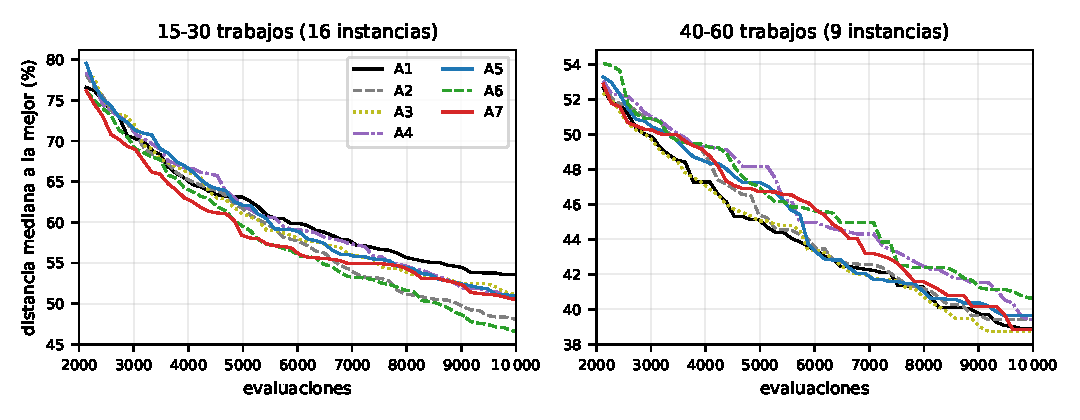
\includegraphics[width=\linewidth]{figuras/convergencia.pdf}
\caption{Distancia mediana a la mejor aptitud encontrada en la instancia, por cualquier variante,
según el número de evaluaciones. La mediana se toma sobre todas las corridas e instancias de
cada grupo de tamaño. Se omiten las primeras 2000 evaluaciones, en las que todas las variantes
coinciden.}
\label{fig:conv}
\end{figure}

\paragraph{P2: aprender la intensidad.}
Aprender la intensidad no aporta. A5 queda un 0,60~\% por encima de A2 y pierde en 16 de 25
instancias ($p=0\dc16$). Frente a la elección aleatoria (A3) y al control por reglas (A4), las
diferencias no superan el 0,8~\%. La causa está en la señal de recompensa. En A5 y A7, el 88~\%
de los bloques termina sin mejora y entrega recompensa nula. Además, en A3, que elige $p$ al
azar, las tres intensidades producen casi la misma recompensa media por bloque: $3\dc78$,
$3\dc61$ y $3\dc60\times10^{-3}$ para $p=0\dc05$, $0\dc15$ y $0\dc30$. O sea, no existe una
intensidad mejor que aprender. El bandido se fija en una intensidad dentro de cada corrida y la
usa en el 69~\% de los bloques, pero cuál elige es casi azar: cada valor domina en un 31 a 37~\%
de las corridas. En la práctica, A5 se comporta como A3. El control por reglas, en cambio,
interpreta la falta de mejora como una señal para subir la intensidad. Desde el tercio medio de
la corrida usa $p=0\dc30$ en más del 90~\% de los bloques, por lo que se asemeja a A2.

\paragraph{P3: aprender el movimiento.}
Aprender el movimiento tampoco mejora $f$ de forma apreciable. A6 y A2 difieren un 0,25~\%
($p=0\dc96$) y A7 queda un 0,26~\% por encima de A5 ($p=0\dc79$). A6 obtiene el mejor rango
promedio (3,08), pero su ventaja frente a A2 se reparte casi por igual entre las instancias. A7
no supera a ninguna variante. Su diferencia más marcada es frente a A6 (+1,16~\%, 18 instancias
perdidas, $p_{\text{Holm}}=0\dc45$), y en las instancias de 40 a 60 trabajos obtiene el peor
rango (5,33). A diferencia del nivel de intensidad, este nivel sí aprende algo. Su señal es más
densa, porque cada mutación produce una observación. Al final de la corrida, $V(m)$ vale en
promedio 0,42 para el intercambio y la inserción, y 0,38 para el cambio de sala. Así, el
bandido reduce el uso del cambio de sala del 33~\% en A2 al 25~\% en A6 y al 28~\% en A7. Esa
preferencia es consistente, pero la diferencia entre movimientos es pequeña y no alcanza a
cambiar el resultado.

\paragraph{Qué cambia en el calendario.}
Las mejoras en $f$ no provienen de un calendario más compacto. En A1, el término de esperas
$\beta\sum_j W_j$ representa en mediana el 62~\% de $f$, frente al 22~\% de $\Cmax$, el 13~\% de
la espera máxima y el 3~\% del balance de salas. La mutación reduce sobre todo la espera total:
un 6,0~\% en A6 y un 4,2~\% en A2 respecto de A1 (Tabla~\ref{tab:res}). A cambio, $\Cmax$ aumenta
hasta un 1,3~\%, y A1 obtiene el mejor rango en $\Cmax$ (3,40). Esto confirma la advertencia de
la Sección~\ref{sec:prob}: una reducción de $f$ puede no traducirse en una jornada más corta. Además, la
espera máxima mediana es de unos 125 minutos en todas las variantes. Ese valor supera el límite
de 27 a 53 minutos que declaran las instancias, porque el evaluador no lo aplica
(Sección~\ref{sec:exp}). Por tanto, los calendarios obtenidos no respetarían ese límite clínico.

\paragraph{Costo, estabilidad y sensibilidad.}
El control es barato. La mediana del cociente entre el tiempo de cada variante y el de A1, con la
misma instancia y semilla, va de 1,004 a 1,008. Una corrida tarda entre 2,1~s (15 trabajos) y
6,8~s (60 trabajos), y la prueba completa tomó 31 minutos. En cambio, ninguna variante mejora la
estabilidad. El rango intercuartílico relativo es del 12,4~\% en A1 y de 13,6 a 15,8~\% en las
variantes con mutación. Por último, el análisis de sensibilidad en desarrollo no muestra
dependencia de los parámetros del control. Con $L\in\{3,10\}$ y $\epsilon\in\{0\dc05;\,0\dc2\}$,
A7 difiere de su configuración base entre $-2\dc2$ y $+1\dc1$~\% en mediana, y la prueba de
Friedman no detecta diferencias ($p=0\dc33$).

\paragraph{Discusión.}
El diseño suponía que la intensidad útil cambia a lo largo de la búsqueda, como ocurre con los
operadores en los trabajos de selección adaptativa~\cite{fialho2010}. En este problema no se
observa: las tres intensidades producen la misma mejora por bloque durante toda la corrida.
Fialho et~al.~\cite{fialho2010} destacan que la selección de operadores es un problema dinámico.
Nuestros resultados agregan una condición previa: si las opciones no difieren, no hay nada que
seguir. La
ablación permite atribuir la pequeña ganancia observada a añadir perturbación y no a aprender a
elegirla. Sin ese diseño, la mejora de A6 sobre A1 (1,6~\%) podría haberse leído como un aporte
del aprendizaje. Para el diseño de controles aprendidos, la implicación práctica es comprobar
primero, con una variante aleatoria como A3, que las opciones producen efectos distinguibles.

\section{Conclusión}

La planificación de cirugías electivas exige coordinar el orden de atención y las salas bajo
recursos compartidos. La literatura ha aprendido qué operador aplicar en algoritmos evolutivos,
pero no había estudiado el aprendizaje de la intensidad y del tipo de perturbación en un enjambre
discreto aplicado a este problema. Propusimos un control en dos niveles para dPSO y lo evaluamos
con una ablación, el mismo presupuesto y separación entre instancias de desarrollo y de prueba.

Los resultados no muestran diferencias significativas entre las siete variantes. Añadir mutación
reduce la aptitud mediana un 1~\%, y un 3~\% en las instancias de 15 a 30 trabajos, sobre todo
porque disminuye las esperas. Aprender la intensidad no aporta, porque las tres intensidades
producen la misma mejora por bloque. Aprender el movimiento identifica que el cambio de sala
mejora con menos frecuencia, pero esa diferencia no se traduce en mejores soluciones. El control
añade menos del 1~\% de tiempo de ejecución. El aporte del trabajo es, por tanto, un resultado
negativo informativo: separa el efecto de perturbar del efecto de aprender a perturbar y muestra
por qué el segundo no aparece.

\paragraph{Limitaciones.}
Las instancias son sintéticas y deterministas, por lo que las conclusiones no se extienden a
datos hospitalarios ni a duraciones inciertas. La función objetivo está dominada por la suma de
esperas, y el evaluador no aplica el límite de espera de cada instancia. El presupuesto de
$10\,000$ evaluaciones no basta para que la búsqueda converja en las instancias de 40 a 60
trabajos. La recompensa de ambos niveles incluye el efecto del paso de dPSO. Por último, la
comparación es interna a dPSO.

\paragraph{Trabajo futuro.}
Tres líneas siguen de estos resultados. La primera es corregir el evaluador para que aplique el
límite de espera de cada instancia y revisar los pesos de $f$. La segunda es dar al nivel de
intensidad opciones con efectos más distintos y una recompensa más densa, por ejemplo por
partícula o basada en rangos, como en Li et~al.~\cite{li2014}. La tercera es evaluar con
presupuestos mayores en las instancias grandes y comparar con las otras metaheurísticas del
repositorio. En una perspectiva más amplia, un control aprendido solo puede aportar si las
opciones que elige producen efectos distinguibles. Comprobarlo con una variante aleatoria es
barato y debería preceder al diseño de cualquier control de este tipo.

\begin{thebibliography}{99}\small
\setlength{\itemsep}{2pt}

\bibitem{cardoen2010} Cardoen, B.; Demeulemeester, E.; Beliën, J. Operating room planning and
scheduling: A literature review. \emph{European Journal of Operational Research} \textbf{2010},
201(3), 921--932. doi:10.1016/j.ejor.2009.04.011.

\bibitem{samudra2016} Samudra, M.; Van Riet, C.; Demeulemeester, E.; Cardoen, B.; Vansteenkiste, N.;
Rademakers, F.E. Scheduling operating rooms: achievements, challenges and pitfalls.
\emph{Journal of Scheduling} \textbf{2016}, 19(5), 493--525. doi:10.1007/s10951-016-0489-6.

\bibitem{pham2008} Pham, D.-N.; Klinkert, A. Surgical case scheduling as a generalized job shop
scheduling problem. \emph{European Journal of Operational Research} \textbf{2008}, 185(3),
1011--1025. doi:10.1016/j.ejor.2006.03.059.

\bibitem{bai2022} Bai, X.; Zhang, W.; Luo, L.; Ma, H.; Zhu, T. Day Surgery Scheduling and
Optimization in Large Public Hospitals in China: A Three-Station Job Shop Scheduling Problem.
\emph{Journal of Healthcare Engineering} \textbf{2022}, 2022, 1149657. doi:10.1155/2022/1149657.

\bibitem{baesler2015} Baesler, F.; Gatica, J.; Correa, R. Simulation optimisation for operating room
scheduling. \emph{International Journal of Simulation Modelling} \textbf{2015}, 14(2), 215--226.
doi:10.2507/IJSIMM14(2)3.287.

\bibitem{eiben1999} Eiben, A.E.; Hinterding, R.; Michalewicz, Z. Parameter control in evolutionary
algorithms. \emph{IEEE Transactions on Evolutionary Computation} \textbf{1999}, 3(2), 124--141.
doi:10.1109/4235.771166.

\bibitem{karafotias2015} Karafotias, G.; Hoogendoorn, M.; Eiben, A.E. Parameter Control in
Evolutionary Algorithms: Trends and Challenges. \emph{IEEE Transactions on Evolutionary
Computation} \textbf{2015}, 19(2), 167--187. doi:10.1109/TEVC.2014.2308294.

\bibitem{aleti2016} Aleti, A.; Moser, I. A Systematic Literature Review of Adaptive Parameter
Control Methods for Evolutionary Algorithms. \emph{ACM Computing Surveys} \textbf{2016}, 49(3),
1--35. doi:10.1145/2996355.

\bibitem{thierens2005} Thierens, D. An adaptive pursuit strategy for allocating operator
probabilities. En \emph{Proceedings of the 7th Annual Conference on Genetic and Evolutionary
Computation}; ACM, \textbf{2005}; pp.~1539--1546. doi:10.1145/1068009.1068251.

\bibitem{dacosta2008} DaCosta, L.; Fialho, Á.; Schoenauer, M.; Sebag, M. Adaptive operator
selection with dynamic multi-armed bandits. En \emph{Proceedings of the 10th Annual Conference on
Genetic and Evolutionary Computation}; ACM, \textbf{2008}; pp.~913--920.
doi:10.1145/1389095.1389272.

\bibitem{fialho2010} Fialho, Á.; Da Costa, L.; Schoenauer, M.; Sebag, M. Analyzing bandit-based
adaptive operator selection mechanisms. \emph{Annals of Mathematics and Artificial Intelligence}
\textbf{2010}, 60(1--2), 25--64. doi:10.1007/s10472-010-9213-y.

\bibitem{li2014} Li, K.; Fialho, Á.; Kwong, S.; Zhang, Q. Adaptive Operator Selection With Bandits
for a Multiobjective Evolutionary Algorithm Based on Decomposition. \emph{IEEE Transactions on
Evolutionary Computation} \textbf{2014}, 18(1), 114--130. doi:10.1109/TEVC.2013.2239648.

\bibitem{shi2001} Shi, Y.; Eberhart, R.C. Fuzzy adaptive particle swarm optimization. En
\emph{Proceedings of the 2001 Congress on Evolutionary Computation}; IEEE, \textbf{2001}; vol.~1,
pp.~101--106. doi:10.1109/CEC.2001.934377.

\bibitem{ratnaweera2004} Ratnaweera, A.; Halgamuge, S.K.; Watson, H.C. Self-Organizing Hierarchical
Particle Swarm Optimizer With Time-Varying Acceleration Coefficients. \emph{IEEE Transactions on
Evolutionary Computation} \textbf{2004}, 8(3), 240--255. doi:10.1109/TEVC.2004.826071.

\bibitem{zhan2009} Zhan, Z.-H.; Zhang, J.; Li, Y.; Chung, H.S.-H. Adaptive Particle Swarm
Optimization. \emph{IEEE Transactions on Systems, Man, and Cybernetics, Part B (Cybernetics)}
\textbf{2009}, 39(6), 1362--1381. doi:10.1109/TSMCB.2009.2015956.

\bibitem{samma2016} Samma, H.; Lim, C.P.; Mohamad Saleh, J. A new Reinforcement Learning-based
Memetic Particle Swarm Optimizer. \emph{Applied Soft Computing} \textbf{2016}, 43, 276--297.
doi:10.1016/j.asoc.2016.01.006.

\bibitem{kennedy1997} Kennedy, J.; Eberhart, R.C. A discrete binary version of the particle swarm
algorithm. En \emph{1997 IEEE International Conference on Systems, Man, and Cybernetics}; IEEE,
\textbf{1997}; vol.~5, pp.~4104--4108. doi:10.1109/ICSMC.1997.637339.

\bibitem{talbi2021} Talbi, E.-G. Machine Learning into Metaheuristics: A Survey and Taxonomy.
\emph{ACM Computing Surveys} \textbf{2021}, 54(6), 1--32. doi:10.1145/3459664.

\bibitem{karimi2022} Karimi-Mamaghan, M.; Mohammadi, M.; Meyer, P.; Karimi-Mamaghan, A.M.;
Talbi, E.-G. Machine learning at the service of meta-heuristics for solving combinatorial
optimization problems: A state-of-the-art. \emph{European Journal of Operational Research}
\textbf{2022}, 296(2), 393--422. doi:10.1016/j.ejor.2021.04.032.

\bibitem{sutton2018} Sutton, R.S.; Barto, A.G. \emph{Reinforcement Learning: An Introduction},
2.\textsuperscript{a}~ed.; MIT Press, \textbf{2018}; cap.~2. ISBN: 9780262039246.

\bibitem{derrac2011} Derrac, J.; García, S.; Molina, D.; Herrera, F. A practical tutorial on the use
of nonparametric statistical tests as a methodology for comparing evolutionary and swarm
intelligence algorithms. \emph{Swarm and Evolutionary Computation} \textbf{2011}, 1(1), 3--18.
doi:10.1016/j.swevo.2011.02.002.

\end{thebibliography}

\end{document}
